%
% THE BEER-WARE LICENSE (Rev. 42):
% Ronny Bergmann <bergmann@mathematik.uni-kl.de> wrote this file. As long as you
% retain this notice you can do whatever you want with this stuff. If we meet
% some day, and you think this stuff is worth it, you can buy me a beer or
% coffee in return.
%
% This file is just to get started - You need the corresponding Logo
%


%\documentclass[german,10pt,xcolor=colortbl,compress
%,draft
%]{beamer}
\documentclass[german,10pt,xcolor=colortbl,compress]{beamer}
\usepackage[utf8x]{inputenc}
\usepackage[OT1]{fontenc}
\usepackage{calc}
\usepackage{csquotes} % automatic quotes
\usepackage[english]{babel}
\usepackage{amsmath,amsthm,amssymb,euscript} % AMS-LaTeX
\usepackage{enumerate,graphicx}
%\usepackage{listings}
\usepackage{tikz}

% Load Theme
\usetheme[noptsans,navigation=true, FB=Mathematik, frametotal=true]{TUKL}
%
\setbeamertemplate{navigation symbols}{}
\title{Real root isolation}
\subtitle{Fachpraktikum}
\date{\today}
\author{Dominik Bendle \and Clara Petroll}
\institute{AG Algebra, Geometrie und Computeralgebra \\ Supervisor: Janko Böhm}
%Setze ein Logo auf der Titelseite unten rechts
%\renewcommand{\theSecondLogo}{}

\begin{document}
\maketitle
\begin{frame}{Contents}
    \tableofcontents
\end{frame}

\section{Introduction}
\begin{frame}{Problem}
    \begin{itemize}
        \item Given: zero-dimensional radical ideal $J \subseteq \mathbb{R}[x_1, \hdots,
            x_n]$ and a box  $B=I_1 \times \cdots \times I_n$, where $I_i$ are real
            intervals for $i=1,\hdots,n$.
        \item Find boxes $B_i \subseteq B$, such that any box contains exactly one element
            of $V(J)$.
    \end{itemize}
    \pause

    Why does this task make sense?
    \begin{lemma}
        Let $J \subseteq \mathbb{R}[x_1, \hdots, x_n]$ be an ideal. Then the following are
        equivalent:
        \begin{enumerate}[a)]
            \item $J$ is zero-dimensional.
            \item $V(J)$ is finite.
        \end{enumerate}
    \end{lemma}
\end{frame}

\begin{frame}{Approach}
    \begin{itemize}
    \item interval arithmetic and exclusion to find out if there is no solution in a box
    \item multivariate Interval Newton step to get uniqueness of a solution in a box
    \item implementation in a Singular library
    \end{itemize}
\end{frame}

\section{Algorithm}
\begin{frame}{Interval arithmetic}
    \begin{definition}
    Let $[x_1,x_2], [y_1,y_2]$ be real intervals. Then the elementary operations of interval arithmetic are defined as follows:
        \begin{itemize}
            \item Addition: $[x_1,x_2] + [y_1,y_2] = [x_1+y_1,x_2+y_2]$
            \item Subtraction: $[x_1,x_2] - [y_1,y_2] = [x_1-y_2,x_2-y_1]$
            \item Multiplication: $[x_1,x_2] \cdot [y_1,y_2] = [\min(x_1y_1,x_1y_2,x_2y_1,x_2y_2), \max(x_1y_1,x_1y_2,x_2y_1,x_2y_2)]$
            \item Division: \\ $[x_1,x_2] / [y_1,y_2] = [x_1,x_2] \cdot 1/[y_1,y_2]$ \\where $1/[y_1,y_2]= [1/y_1, 1/y_2]$ if $0 \notin [y_1,y_2] $
        \end{itemize}
    \end{definition}
\end{frame}

\begin{frame}{Interval arithmetic}
    Further, as calculating $[x_1,x_2]^n = [x_1, x_2] \cdots [x_1,. x_2]$ generally yields a
    loose bound it makes sense to define interval powers separately:
    \begin{definition}
        Let $I := [x_1, x_2]$ be a real interval, then the powers of $I$ are defined
        as
        \begin{align*}
            I^n =
            \begin{cases}
                [x_1^n, x_2^n] & \text{if $n$ odd or $x_1 > 0$,} \\
                [x_2^n, x_1^n] & \text{if $n$ even and $x_2 < 0$,} \\
                [0, \max(x_1^n, x_2^n)] & \text{else, i.e. if $n$ even and $0\in I$.}
            \end{cases}
        \end{align*}
    \end{definition}
\end{frame}

\begin{frame}{Interval arithmetic}
    \begin{definition}
        Let  $\mathbf{R} \subseteq \mathbb{R}^2$ be the set of all real intervals $[a,b],
        a < b$. An interval extension of a map $g: \mathbb{R}^n \to \mathbb{R}$ is a map
        $\mathbf{g}: \mathbf{R}^n \to \mathbf{R}$ such that $g(x) \in
        \mathbf{g}(\mathbf{x}) $ for all $x \in \mathbb{R}$.
    \end{definition}

    This allows us to perform a simple exclusion test using interval arithmetic.
    \bigskip

    \emph{Problem:} How do we get uniqueness of a solution in a box?
\end{frame}

\begin{frame}{Interval Newton Step}
    \begin{itemize}
    \item Idea: We want to have a test $T$, which for a given map $f: \mathbb{R}^n \to
        \mathbb{R}^n$ and a given box $B_i$ returns:
        \begin{itemize}
            \item $T(f,B_i)=-1$, if there is no $x \in B_i$ such that $f(x)=0$.
            \item $T(f,B_i)=1$,  if there is a unique $x \in B_i$ such that $f(x)=0$.
            \item $T(f,B_i)=0$, else.
        \end{itemize}
    \end{itemize}
    \pause
    To get this, we compute the interval Newton step of $f$ and a box $\mathbf{x}$: $$
    N(f, \mathbf{x})= \hat{x} - \mathbf{f'}(\mathbf{x})^{-1}f(\hat{x})$$ where $\hat{x}
    \in \mathbf{x}$ arbitrary point, $\mathbf{f'}$ the interval extension of the Jacobian
    matrix of $f$.
\end{frame}

% Vllt beispiel bei dem matrix invertiert wird??
\begin{frame}{Interval Newton step}
    \begin{theorem}
        Let $\mathbf{x}$ be a box in $\mathbb{R}^n$ and $f:\mathbb{R}^n\to \mathbb{R}^n$.
        Then it holds:
        \begin{enumerate}[a)]
            \item Every solution in $\mathbf{x}$ is also in $N(f,\mathbf{x})$.
            \item If $N(f,\mathbf{x}) \subseteq int(\mathbf{x})$, then there is a unique
                solution in $\mathbf{x}$, i.e. $T(f,\mathbf{x})=1$.
        \end{enumerate}
    \end{theorem}
    \pause

    \textbf{Implementation:} \\
    %Bisection until for every of the arising boxes one of the following conditions is satisfied:
    Bisection until every box satisfies one of the following conditions:
    \begin{itemize}
        \item there is exactly one solution in the box
        \item \enquote{size} of the box is below a given bound.
    \end{itemize}
\end{frame}


\begin{frame}{Interval Newton Step}{Application to our problem}
    \begin{theorem}
        Let $I$ be a zero-dimensional radical ideal of $K[x_1, \hdots, x_n]$, where $K$ is
        a field. Then $I$ is generated by $n$ elements.
    \end{theorem}
    \pause

    \begin{itemize}
        \item zero-dimensional radical ideal $I \subseteq \mathbb{R}[x_1, \hdots, x_n]$ is
            therefore given by a set $\{f_1, \hdots f_n\}, f_i \in \mathbb{R}[x_1, \hdots,
            x_n]; i=1,\hdots,n$ of generators.
        \item consider the function
            \begin{equation*}
                f:= \begin{pmatrix} f_1\\ \vdots \\ f_n \end{pmatrix},
                f:\mathbb{R}^n\to \mathbb{R}^n
            \end{equation*}
    \end{itemize}
    $\implies$ We can apply the interval Newton step to our ideal.
\end{frame}

\section{Problems \& Improvements}
\begin{frame}{Bad run time}
    \begin{itemize}
        \item interval arithmetic implemented as a \enquote{newstruct} in Singular
        \item inverting of an interval matrix difficult
    \end{itemize}
    \bigskip
    \pause
    \textbf{Our improvements:}
    \pause
    \begin{itemize}
        \item outsourcing of the interval arithmetic in C++ (dynamic modules in Singular)
        \item integrate this part as .so
        \item inverting of the interval matrices with Gaussian elimination
    \end{itemize}
\end{frame}

\begin{frame}{Gaussian elimination for interval matrices}
    \begin{definition}
    An interval matrix $\mathbf{A}=[A_1,A_2] \in \mathbf{R}^{n \times n} $ where $A_1, A_2 \in \mathbb{R}^{n\times n}$ are the lower and upper bound of the matrix is called regular, if all real matrices $A \in \mathbf{A}$ are regular. Otherwise $\mathbf{A} $ is called singular.\\
    An interval matrix B is called an inverse of a regular interval matrix $\mathbf{A} $ if it contains the inverse of each real matrix $A \in \mathbf{A}$.

    %An interval matrix $A$ is nonsingular if it doesn't contain a singular matrix.
    \end{definition}
    \pause
    We can invert regular interval matrices with Gaussian elimination:\\
    For example, invert the matrix
    \[
    \left[
    \begin{array}{cc}
    [1,2]&[2,3] \\

    [0,0]&[2,3]\\
    \end{array}
    \right]
    \]

\end{frame}

\begin{frame}
\[
    \left[
    \begin{array}{cc|cc}
    [1,2]&[2,3]&[1,1]&[0,0]  \\

    [0,0]&[2,3]&[0,0]&[1,1]  \\
    \end{array}
    \right]
    \]

    \pause

    $\xrightarrow[\text{}]{\text{'2.row' $ \div  [2,3]$}}$
    \[
    \left[
    \begin{array}{cc|cc}
    [1,2]&[2,3]&[1,1]&[0,0]  \\

    [0,0]&[1,1]&[0,0]&[1/3,1/2]  \\
    \end{array}
    \right]
    \]

    \pause

    $\xrightarrow[\text{}]{\text{'1.row' $ - [2,3]\cdot$'2.row'}}$
    \[
    \left[
    \begin{array}{cc|cc}
    [1,2]&[0,0]&[1,1]&[-3/2,-2/3]  \\

    [0,0]&[1,1]&[0,0]&[1/3,1/2]  \\
    \end{array}
    \right]
    \]

    \pause

    $\xrightarrow[\text{}]{\text{'1.row' $\div  [1,2]$}}$
    \[
    \left[
    \begin{array}{cc|cc}
    [1,1]&[0,0]&[1/2,1]&[-3/2,-1/3]  \\

    [0,0]&[1,1]&[0,0]&[1/3,1/2]  \\
    \end{array}
    \right]
    \]


\end{frame}

\begin{frame}{Big fractions}
    \begin{itemize}
        \item intersecting boxes $\rightarrow$ sometimes really big fractions $\rightarrow$ slow
        \item Idea: \enquote{round} the boxes
        \item Realization: increase the size of the box a little bit, to get nicer fractions.
    \end{itemize}
    \bigskip
    \pause

    \begin{center}
        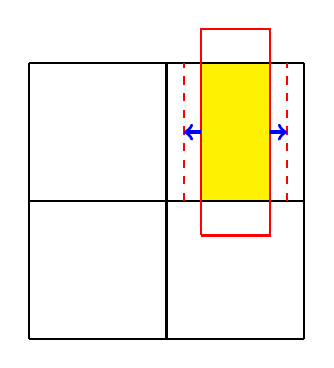
\begin{tikzpicture}[scale=1.75]
            \fill [color=yellow]  (1.25,1) rectangle (1.75,2);
            \draw[thick] (0,0) grid [step=1]     (2,2);
            \draw[thick,red] (1.25,0.75) -- (1.25,2.25)-- (1.75,2.25) -- (1.75, 0.75) -- (1.25,0.75);
            \draw[dashed, red, thick] (1.125,1) -- (1.125,2);
            \draw[dashed, red, thick] (1.875,1) -- (1.875,2);
            \draw [->, very thick, blue] (1.25, 1.5) -- (1.125,1.5);
            \draw [<-, very thick, blue] (1.875,1.5) -- (1.75,1.5);
        \end{tikzpicture}
    \end{center}
    \pause

    $\implies$ This results in acceptable run time even for five variables.
\end{frame}

\begin{frame}{Bad starting boxes}
    \begin{lemma}
        Let $I$ be an ideal of the polynomial ring $K[x_1, \hdots, x_n]$, where $K$ is a
        field. Then the following are equivalent:
        \begin{enumerate}[a)]
            \item $I$ is zero-dimensional.
            \item $I \cap K[x_i] \neq \{0\}$ for $i=1,\hdots, n$.
        \end{enumerate}
    \end{lemma}
    \pause

    \begin{itemize}
        \item Compute Gröbner basis of the ideal with an elimination ordering.
        \item[] $\implies$ First equation only depends of one variable.
        \pause
        \item Apply our exclusion test on this equation $\rightarrow$ we get better
            starting boxes for this variable.
        \item Do this for all variables (by permuting the variables).
        \item Take the Cartesian product of all those boxes as starting boxes.
    \end{itemize}
\end{frame}

\begin{frame}{Boxes with unique solutions}
    \begin {itemize}
        \item So far: Input consisting of an ideal, starting box and a bound for the size
            of the boxes.
        \item[]$\rightsquigarrow$ \emph{Aim:} No boxes should be returned due to the size
            constraint
    \end{itemize}
    \pause
    \textbf{Our improvements:}
    \begin{itemize}
        \item If there is a zero on the plane, at which we want to divide the box for
            bisection $\implies$ wouldn't get uniqueness of the solution with interval
            Newton step.
        \item Same problem if we have a zero on the boundary of the starting box.
        \item Improve our algorithm \texttt{splitBox} by:
        \begin{itemize}
            \item evaluate the ideal at the intersection plane
            \item Gröbner basis test
        \end{itemize}
    \end{itemize}
\end{frame}

\section{Future Improvements}

\begin{frame}{Underlying number type}
    \begin{itemize}
        \item Currently use Singular's \texttt{number} type for easy integration into the
            interpreter
        \item may use floating point numbers instead for increasing speed
            \begin{itemize}
                \item would allow using existing interval arithmetic libraries (MPFR,
                    \dots), however:
                \item requires conversion between Singular number types and C++ number
                    types
                \item may require adaptively changing precision for certain problems
            \end{itemize}
    \end{itemize}
\end{frame}

\begin{frame}
    \begin{itemize}
        \item Extension to interval division: in one-dimensional case it makes sense to
            define $1/[x_1, x_2] = (-\infty, 1/x_1] \cup [1/x_2, \infty)$ if $x_1 < 0 <
            x_2$
        \item[]$\rightarrow$ intervals stay finite since we intersect afterewards
        \item[]$\rightarrow$ Newton step converges to two separate roots
        \item may in some cases allow matrix inversion to succeed more often
        \item However: representing $\infty$ in intermediate steps requires special
            handling in the implementation
    \end{itemize}
\end{frame}

%Literatur

\begin{frame}{Bibliography}
    \bibliographystyle{alphadin}
    \begin{thebibliography}{9}
        \bibitem{Moore} Cloud, Kearfott, Moore
            \textit{Introduction to Interval Analysis}.
            Society for Industrial and Applied Mathematics, 2009.


        \bibitem{Vasconcelos} Eisenbud, Grayson, Herzog, Stillman, Vasconcelos
            \textit{Computational Methods in Commutative Algebra and Algebraic Geometry}.
            Springer Verlag Berlin-Heidelberg, 3. edition 2004.

        \bibitem[A]{Sommese} Andrew J. Sommese and Charles W. Wampler
            \textit{The Numerical Solution of Systems of Polynomials}. [\textit{Arising in
            Engineering and Science}].
            World Scientific Publishing Co. Pte. Ltd., 2005.

    \end{thebibliography}
\end{frame}

\end{document}
% vim: spell spelllang=en
